
%%%%%%%%%%%%%%%%%%%%%%% file typeinst.tex %%%%%%%%%%%%%%%%%%%%%%%%%
%
% This is the LaTeX source for the instructions to authors using
% the LaTeX document class 'llncs.cls' for contributions to
% the Lecture Notes in Computer Sciences series.
% http://www.springer.com/lncs       Springer Heidelberg 2006/05/04
%
% It may be used as a template for your own input - copy it
% to a new file with a new name and use it as the basis
% for your article.
%
% NB: the document class 'llncs' has its own and detailed documentation, see
% ftp://ftp.springer.de/data/pubftp/pub/tex/latex/llncs/latex2e/llncsdoc.pdf
%
%%%%%%%%%%%%%%%%%%%%%%%%%%%%%%%%%%%%%%%%%%%%%%%%%%%%%%%%%%%%%%%%%%%


\documentclass[runningheads,a4paper]{llncs}

\usepackage{amssymb}
\setcounter{tocdepth}{3}
\usepackage{graphicx}
\usepackage{epstopdf}
\usepackage[utf8]{inputenc}
\usepackage[T1]{fontenc}
\usepackage{lmodern}

\usepackage{url}
\urldef{\mailsa}\path|loic.tetrel@mail.mcgill.ca|    
\newcommand{\keywords}[1]{\par\addvspace\baselineskip
\noindent\keywordname\enspace\ignorespaces#1}

\begin{document}

\mainmatter  % start of an individual contribution

% first the title is needed
\title{Litterature review : Sensorless registration of echographic images for 3D ultrasound}

% a short form should be given in case it is too long for the running head
\titlerunning{Sensorless registration of echographic images for 3D ultrasound}

% the name(s) of the author(s) follow(s) next
%
% NB: Chinese authors should write their first names(s) in front of
% their surnames. This ensures that the names appear correctly in
% the running heads and the author index.
%
\author{Loïc Tetrel}
%loic.tetrel@mail.mcgill.ca
\authorrunning{Sensorless registration of echographic images for 3D ultrasound}
% (feature abused for this document to repeat the title also on left hand pages)

% the affiliations are given next; don't give your e-mail address
% unless you accept that it will be published
\institute{McGill University\\
845 Rue Sherbrooke O, QC H3A 0G4, Montréal, Canada\\
\mailsa\\
}

%\toctitle{Sensorless registration of echographic images for 3D ultrasound}
\maketitle

\begin{abstract}
The purpose of this paper is to summarize the main contributions in the area of sensorless registration for 3D echography. Because the registration is performed using the echographic noise called speckle, the problematic is really complex due to the nature of speckle in ultrasound. We will see that the registration of echographic images has to be performed by dividing the main problem in the estimation of out-of-plane ($z, \theta_x, \theta_y$) and in-plane ($x, y, \theta_z$) parameters. This will lead to many discussion like the influence on the rotation of the probe, the question of real tissue imagery and the reconstruction of the frame's  pose.
\keywords{3D ultrasound. Statistics of speckle. RF signal. Sensorless rigid registration.}
\end{abstract}

\section{Introduction}

Echography is an imaging modality that has been widely used thanks to its many benefits : cheapness, flexibility and safety. 
Compare to the traditional 2D echography, 3D echography allows a better evaluation of the anatomical structures and a more specific analysis of the defects.\par
A 3D probe can be used to obtain the 3D echographic volume, but it's expensive and the view is limited by the width of the probe. 
With the traditional 2D equipment, the clinician probes the area of interest by acquiring a sequence of images or frames.
The volumetric reconstruction of this sequence require to obtain the position ($x,y,z,\theta_x, \theta_y, \theta_z$) of all the frames relative to the first one. 
Then a position sensor is fixed to the probe so we can obtain its displacement at a reasonable rate (usually $30 frames/sec$). 
The limitations with this approach are that it cost a lot, it is cumbersome and a calibration is necessary. 
A more difficult method is to use the information of the images itself to perform a sensorless registration of the frames. 
If this information is known during time and/or space, we can use it as a reference in the sequence to registrate all the images of the acquisition. Many research \cite{chen1997determination,tuthill1998automated,wagner1983statistics} investigated the sensorless way to registrate echographic images so the aim of this paper is to abstract the different methods in the litterature. During this review, we will follow a guideline by trying to answer these questions : (i) What is the best information available in echographic images ? (ii) How researchers registrate the frames ? (iii) What are the limitations and difficulties ?

\section{What is the best information available in echographic images ?}

Before trying to answer our question, we need to begin by laying the basis of echographic images.\par
\textbf{Utility of ultrasound} As many know, ultrasound can be used to evaluate the position and thickness of an interference. A piezoelectric element emits a short impulse through the area of interest, then an echo of this impulse will be produced if there is an interference.\par
\textbf{Image creation.} In echography, two modes are widely used : A-mode and B-mode. 
The A-mode signal is just the envelop of the complex signal (called RF signal) measured by one piezoelectric element. 
The B-mode image is created using a transducer with an array of piezoelectric elements. So the delay between the echo and the impulse correspond to the position of the interference (position of the pixel) and the amplitude of the signal correspond to the interference density (grey-value of the pixel).\par
\textbf{Speckle.} When an ultrasonic wave get through one medium to another, there is a reflection, an absorption and a transmission of this wave depending on the medium. 
The reflection is specular (or linear) if the signal's wavelength $\lambda$ is lower than the size of this medium, but if $\lambda$ is upper than the medium the reflection is diffuse. 
Because human tissue isn't a perfectly homogeneous medium, there are many micro-particles (or diffusers) which implies a lot of diffuse reflection. The interference of all the echo from these diffusers will create what we call the speckle, this explain the poor quality in echography. 
This artefact justify the difficulty of echographic image analysis because it is not desired and seen as a noise for many researchers. But in fact, the speckle can be verry informative because it carries a lot of informations, more important there is a connection between the spatial configuration of diffusers and the creation of speckle \cite{wagner1983statistics}. 
Because the speckle isn't random and can be used as a reference between images, it opened a new area of interrest called "speckle-tracking" which will be more explain in the next part.
%\begin{figure}
%\centering
%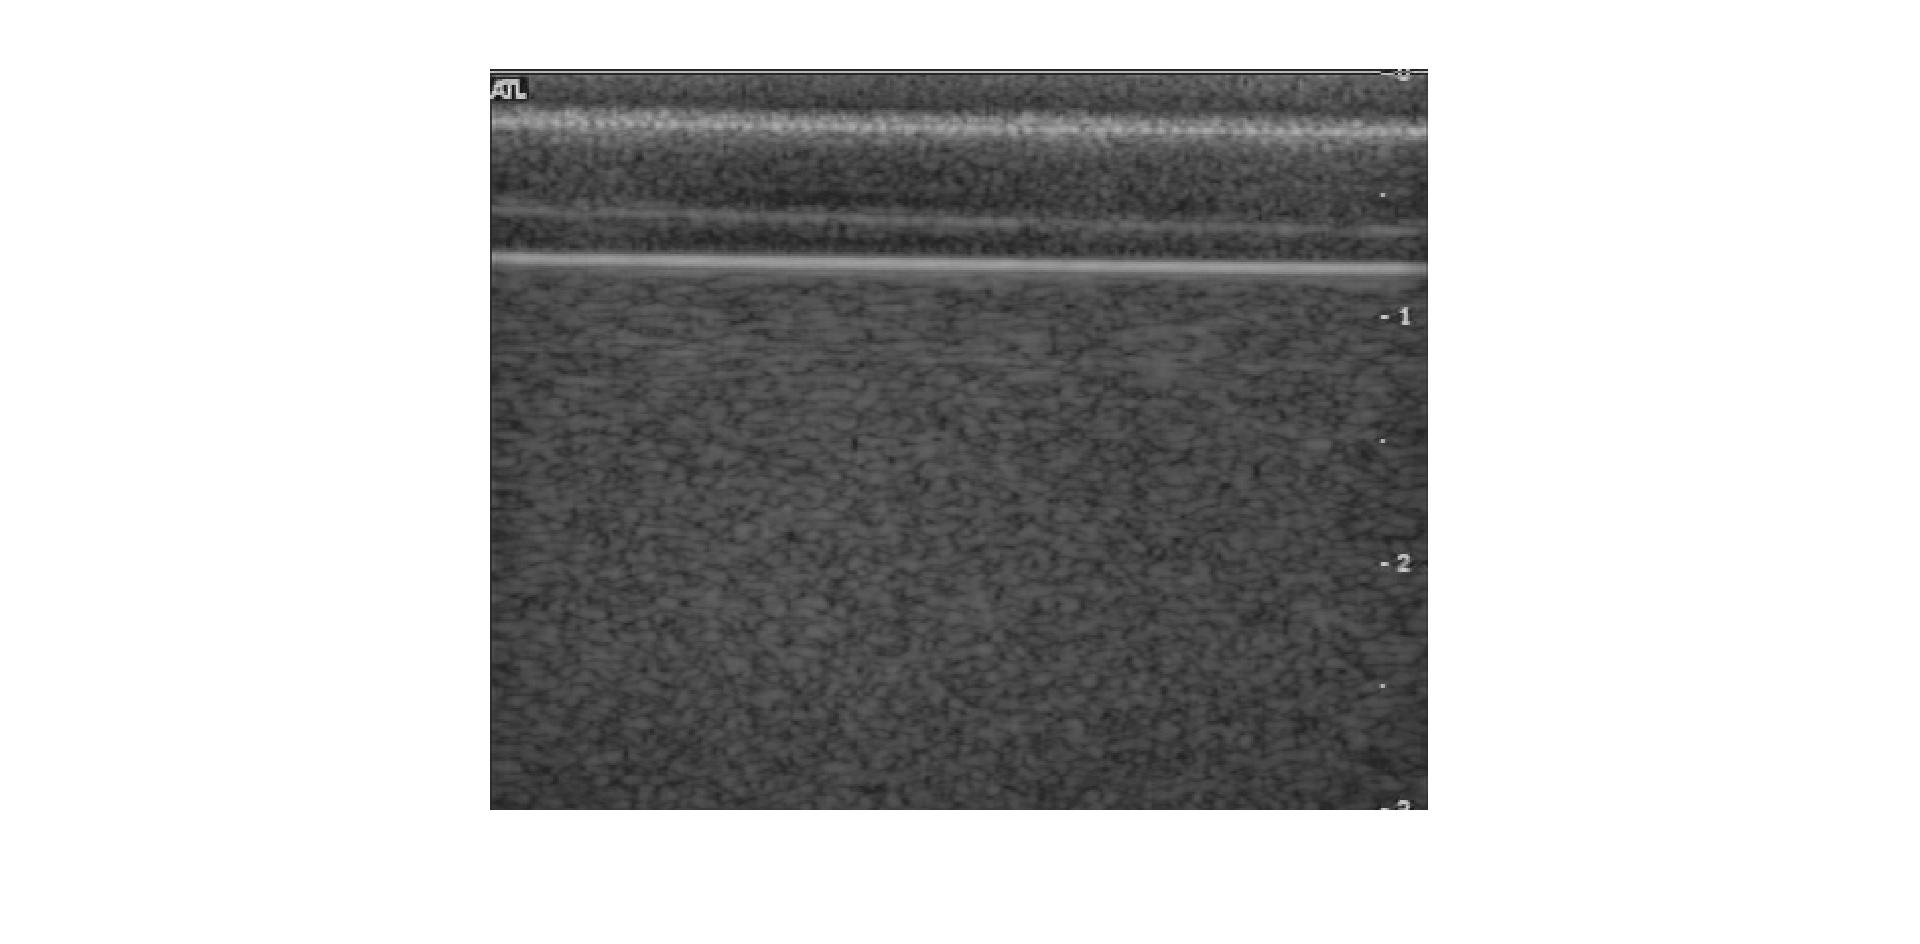
\includegraphics[height=4cm]{Figures/speckle}
%\caption{Interference of the echo from two diffusers (left) (Extracted from \cite{stoylen10}). Echographic image with fully developped speckle from a phantom (right).}
%\label{fig:speckle}
%\end{figure}

\section{How researchers registrate the frames ?}
In the registration for 3D echography, we want to extract the 6 degree of freedom of the motion between two images. We will simplify our problem by just studying the case of rigid transformation, so we hypothetisize that there is just one global motion for two images. When we will talk about elevationnal distance $z$ this will refer to the main movement of the probe outside the image.
%\begin{figure}
%\centering
%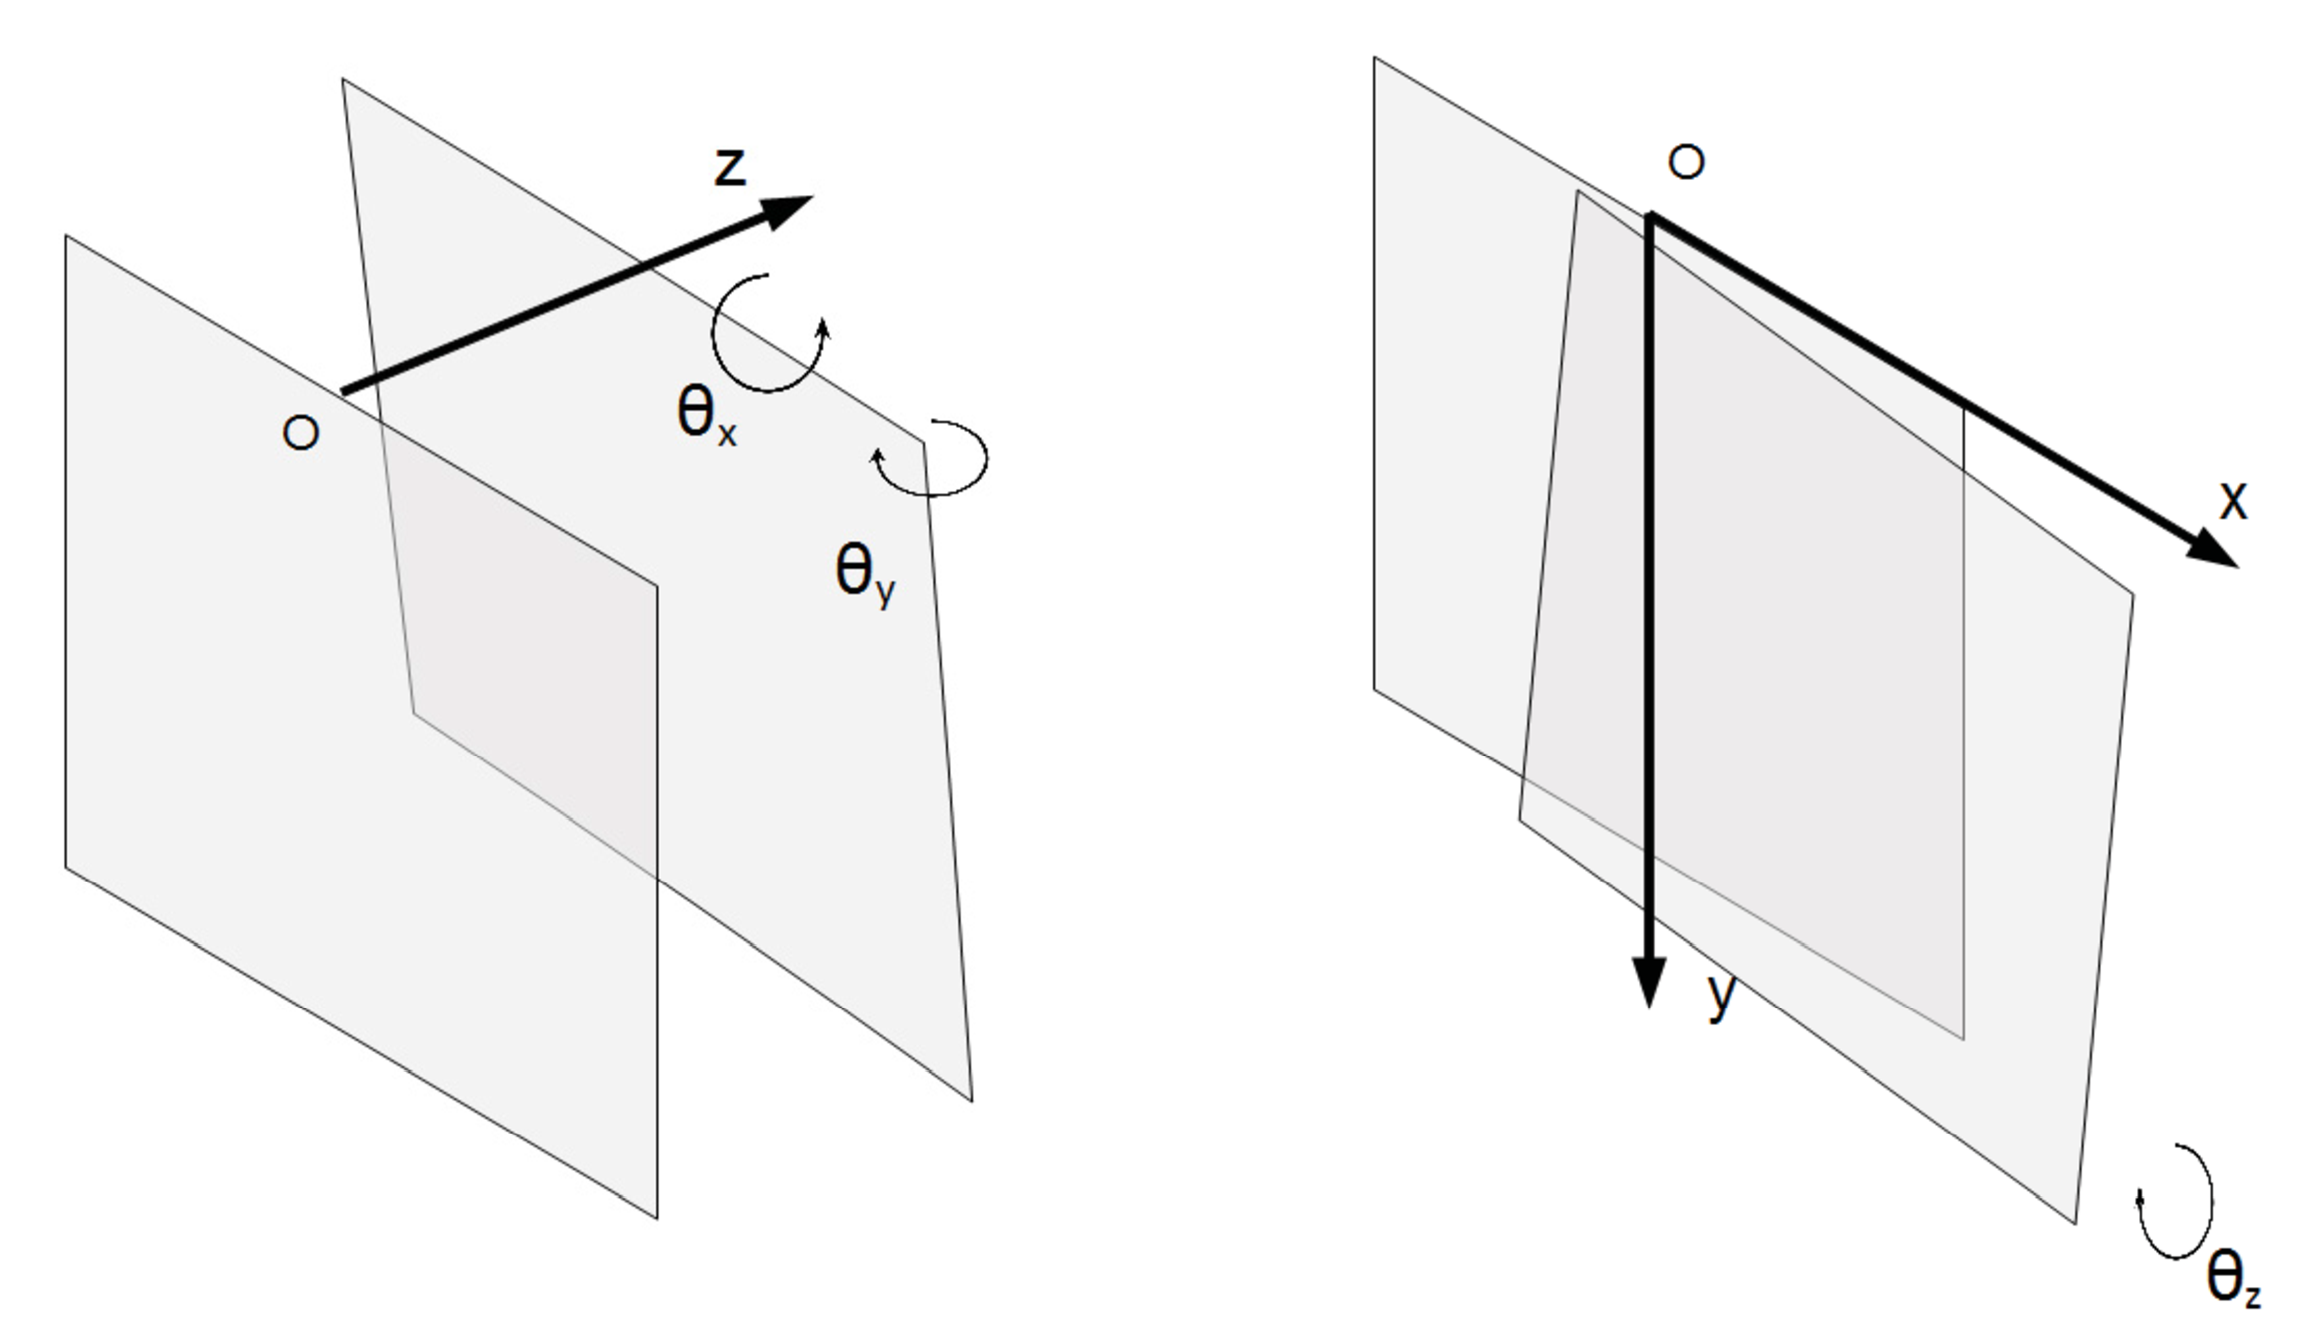
\includegraphics[height=3.5cm]{Figures/mouv_plan}
%\caption{The 6DoF of the probe motion. Out-of-plane motion $z, \theta_x, \theta_y$ (left). In-plane motion $x, y, \theta_z$ (right). (Extracted from \cite{conrath2012recalage})}
%\label{fig:6dof}
%\end{figure}
The case of echography is specific because we extract 6 parameters with 2-dimensionnal images, so usually the problem is
decomposed in the estimation of two motions \cite{tuthill1998automated} : out-of-plane ($z, \theta_x, \theta_y$) and in-plane ($x, y, \theta_z$). We will first focus on the estimation of the in-plane parameters $(x,y)$ and after the out-of-plane parameters $(z)$ specific to 2D echography.\par
\textbf{In-plane estimation $\mathbf{(x,y)}$.} There are two types of sensorless registration : feature-based and intensity-based. With feature-based method, we want to find the same key-points in two images and use them to register despeckled images. 
Schneider \textit{et al.} \cite{schneider2012real} tried to register 3D US volumes in real time using 3D single-invariant feature transfrom method. 
After retrieving the points in the volumes, they are using a final RANSAC algorithm to perform the rigid registration. 
Their algorithm works well in real-time, however they are making the assumption that there is small variation in rotation and translation on the volume which is not true for freehand data. In intensity-based registration we look at the entire image to estimate the motion, speckle is then an information.
The standard way to estimate the in-plane motion is to calculate the correlation between the first image and the second image, then the maximum value of the correlation map gives us the displacement. Because the pixel resolution is usually low, the correlation in images is not enough accurate for the estimation of little motions.
That's why Housden \textit{et al.} \cite{housden2006subsample} extended the method, by interpolating the correlation data threw a gaussian. This addition leads to an improvement of $5\%$ and became the standard way to perform the correlation in echography, despite the computationnal cost of the method because it is image based. 
The work of Rivaz \textit{et al.} \cite{rivaz2008ultrasound} in elastography is a novel approach using the RF signals and a dynamic programming approach. It is relevant because the use of RF signals gives more precise results, the cost-function is more robust to minimums and it is faster. Moreover, they are replacing the standard correlation by a new cost-function which lead to a better signal-noise ratio than the correlation.\par
\textbf{Out-of-plane estimation $\mathbf{(z)}$.} Extracting the out-of-plane parameters of the motion is difficult and more specific to echography.
The conclusion of Wagner \textit{et al.} \cite{wagner1983statistics} allows the construction of what is called a "speckle-decorrelation curve" under the condition of Rayleigh (the diffusers are scattered randomly). Using such a curve, it is possible to extract a distance $\Delta_r$ knowing the second order statistic of the speckle (correlation $R_U$), the point spread function $h$ of the probe and the constant $\zeta_0^2$ which represent the homogeneous distribution of the diffusers :
\begin{equation}
R_U(\Delta r)=	h(-\Delta r)\times \zeta_0^2\otimes h(\Delta r)
\end{equation}
Because the work was theorical, Chen \textit{et al.} \cite{chen1997determination} experimented it by performing the first test on real imagery, and showing concretly how to produce the speckle-decorrelation curve (see Fig. \ref{fig:speckledecorrelation}).
With the hypothesis that the curve is gaussian, they used a bayesian approach $p(\omega|z,\alpha)$ to estimate the parameters $\omega$ of the curve.
They used a robotic arm moving along the elevationnal direction, and perform a battery of test (variating the step-size or number of steps) to show the reliability of the method.
\begin{figure}
\centering
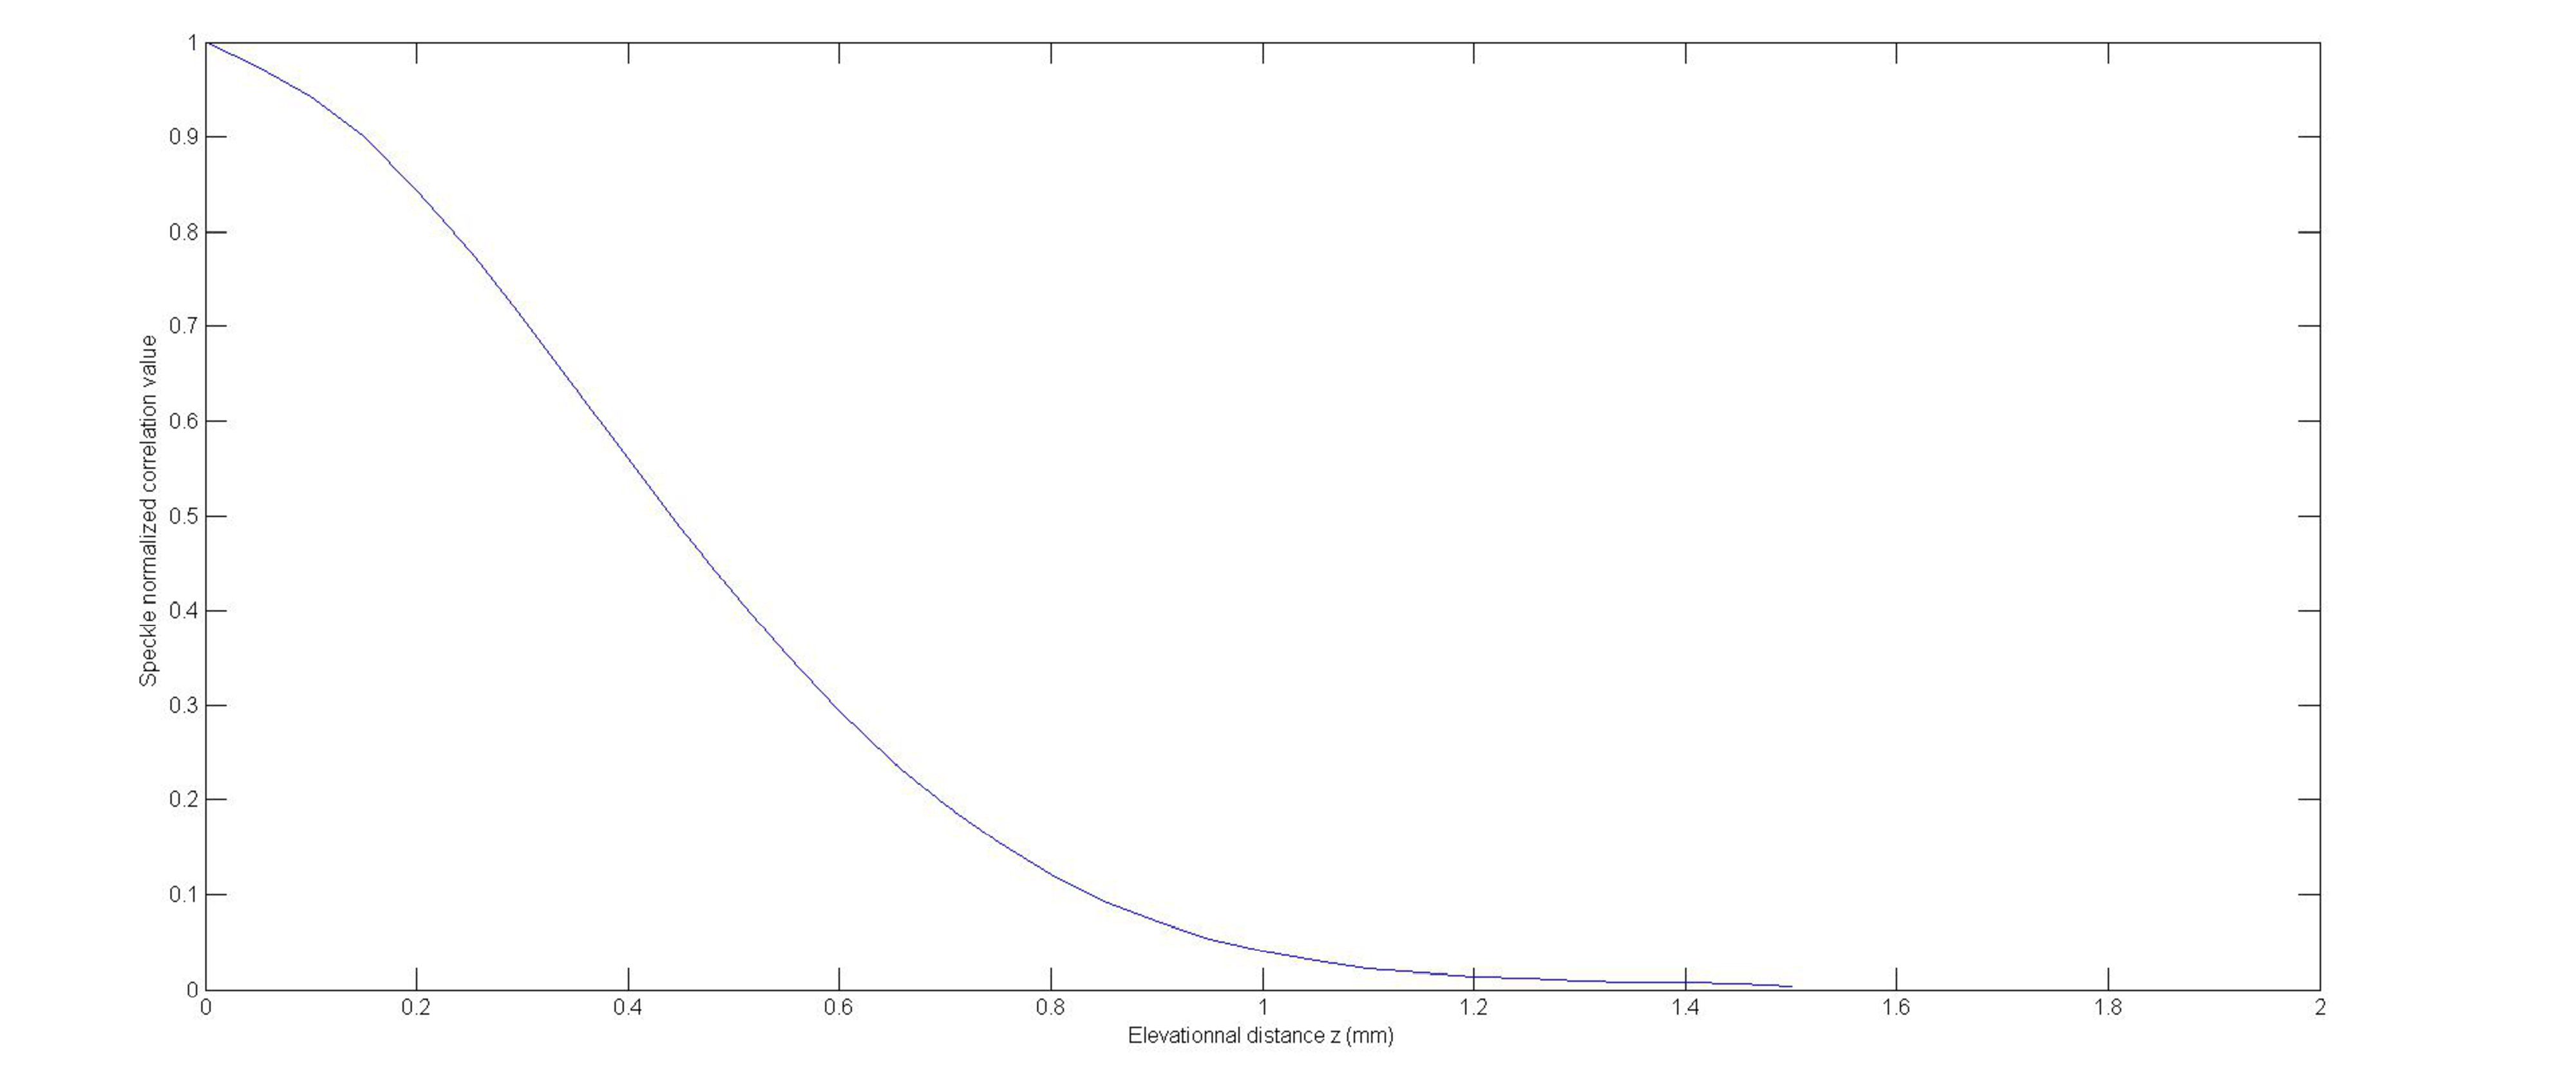
\includegraphics[height=4cm]{Figures/decorrel}
\caption{The relation between the absolute elevationnal distance $z$ and the speckle correlation $\alpha$ of two images.}
\label{fig:speckledecorrelation}
\end{figure}
\par
\textbf{Global rigid registration.} Tuthill \textit{et al.} \cite{tuthill1998automated} where the first to perform the global rigid transformation with speckle decorrelation.They divided the image in different patchs and at the center of each patch $i$ they estimated $(x_i, y_i)$ with the position of the pic in the correlation matrix and extracted $(z_i)$ \cite{chen1997determination}.
Having two cloud of points in both images allowed them to perform a final RANSAC algorithm to estimate the global motion between the two frames. This can be done only with the hypthesis that there is small in-plane rotation $\theta_z$, so the estimation is close to the truth. 
They obtain a $10\%$ position accuracy with this method, but a recent work \cite{conrath2012towards} demonstrated that there is a correlation between the error and the parameters of the motion. 
They used a Relevance Vector Machine (RVM) to correct the error of the estimation. Using inputs-outputs pairs $\{a_i=m_{truth_i}, b_i=m_{estim_i}\}$ they estimated the function $a = f(b)+\epsilon$. Based on a bayesian theory with an initial prior on the weights $p(w)$, they estimated the posterior $p(w|a, b)$.
This leads to a slightly improvement, however this work was performed with simulated images and the speckle doesn't behave in the same way with real images. Moreover, the accuracy depends on the initial prior $p(w)$ which is biased because of the speckle-based estimation.
\section{What are the limitations and difficulties ?}
The problem's complexity involves a lot of difficulties that can be divided in three major groups : (i) rotation, (ii) real tissue, (iii) reconstruction.\par
\textbf{Influence of the rotations.} Kallel \textit{et al.} \cite{kallel1994speckle} are the first to study the influence of the rotation on the speckle, and so in the speckle-decorrelation curve. They demonstrated that the point spread function have a curvature in the direction of wave's propagation when the probe is rotating. This curvature will create some artefacts in the image and as a consequence false the estimation by speckle. That's why all the previous work have low results if they are under big rotations.\par
\textbf{Working on real tissue.} To perform the speckle-decorreation curve, the diffusers has to be under the condition of Rayleigh which is not true for real tissue. Indeed, in real echographic images they are many scatterers like bones, veins, muscle. So the rate of speckle decorrelation is not only transducer dependent, but also medium dependent. This lead to a biased decorrelation curve that Laporte and Arbel \cite{laporte2011learning} tried to correct. Threw a regression-based approach, they extracted the decorrelation curve that suit the best the training data. Using the training data simulated with various speckle images, the results are good compare to the state of the art. However an improvement can be made with a more realistic training data. \par
\textbf{Reconstruction of the frame's position.} To reconstruct the frame's pose relative to the first one, we need to associate many motions because the motion estimated by speckle cannot be to large (see fig. \ref{fig:speckledecorrelation}). This imply an accumulation of error during the reconstruction step, which will bias the estimation of the pose. Till today, all the previous authors have not addressed this issue and many accumulated a lot of errors because of this.

\section{Conclusion}
To conclude this discussion, it is usefull to summarize the main articles that we reviewed. We saw that the out-of-plane estimation was done by using a decorrelation curve \cite{wagner1983statistics}, the in-plane follows the state of the art of registration by serching the position of the pic in the correlation map \cite{housden2006subsample}. 
RF signals can be used to be faster and more precise in the calculation of the correlation \cite{rivaz2008ultrasound}. To perform the global motion estimation with the 6 degree of freedom, a RANSAC regression is a good way \cite{tuthill1998automated}. 
Finally, we can't forget the limitations of the speckle-based estimation by limiting the rotation in the acquisition which will bias our result \cite{kallel1994speckle} and the experimentations with real tissue showed that it's difficult to extract the decorrelation curve \cite{laporte2011learning}.

%\begin{thebibliography}{4}
%
%\bibitem{jour} Smith, T.F., Waterman, M.S.: Identification of Common Molecular
%Subsequences. J. Mol. Biol. 147, 195--197 (1981)
%
%\bibitem{lncschap} May, P., Ehrlich, H.C., Steinke, T.: ZIB Structure Prediction Pipeline:
%Composing a Complex Biological Workflow through Web Services. In: Nagel,
%W.E., Walter, W.V., Lehner, W. (eds.) Euro-Par 2006. LNCS, vol. 4128,
%pp. 1148--1158. Springer, Heidelberg (2006)
%
%\bibitem{book} Foster, I., Kesselman, C.: The Grid: Blueprint for a New Computing
%Infrastructure. Morgan Kaufmann, San Francisco (1999)
%
%\bibitem{proceeding1} Czajkowski, K., Fitzgerald, S., Foster, I., Kesselman, C.: Grid
%Information Services for Distributed Resource Sharing. In: 10th IEEE
%International Symposium on High Performance Distributed Computing, pp.
%181--184. IEEE Press, New York (2001)
%
%\bibitem{proceeding2} Foster, I., Kesselman, C., Nick, J., Tuecke, S.: The Physiology of the
%Grid: an Open Grid Services Architecture for Distributed Systems
%Integration. Technical report, Global Grid Forum (2002)
%
%\bibitem{url} National Center for Biotechnology Information, \url{http://www.ncbi.nlm.nih.gov}
%
%\end{thebibliography}

{\small
\bibliographystyle{splncs03}
\bibliography{review}
}

\end{document}
